\documentclass{article}
\usepackage{tikz}
\usetikzlibrary{matrix, decorations.markings}

% Define styles for arrows and crossings
\tikzset{
    myarrow/.style={->, thick},
    purpleline/.style={ultra thick, purple},
    redline/.style={ultra thick, red},
    crossing/.style={circle, fill=white, inner sep=0pt, minimum size=3pt},
}

\begin{document}

\begin{tikzpicture}[scale=0.8]

% Draw the matrix grid
\matrix (m) [matrix of nodes, column sep=1cm, row sep=1cm, nodes in empty cells] {
    & |(even1)| & |(even2)| & |(even3)| \\
    |(odd1)| & |(odd2)| & |(odd3)| & |(odd4)| \\
};

% Draw horizontal lines between rows and columns
\draw[thick] (m-1-1.north west) -- (m-1-4.north east);
\draw[thick] (m-2-1.south west) -- (m-2-4.south east);
\draw[thick] (m-1-1.west) -- (m-2-1.west);
\draw[thick] (m-1-2.east) -- (m-2-2.east);
\draw[thick] (m-1-3.east) -- (m-2-3.east);
\draw[thick] (m-1-4.east) -- (m-2-4.east);

% Fill in the content

% Even row
\node at (even1) {Even};
\node at (even2) {
    \begin{tikzpicture}[baseline=(current bounding box.center), scale=0.7]
        % Top arrow
        \draw[myarrow] (-1,0) -- (1,0);
        % Vertical line and arrow
        \draw[redline] (0,-1) -- (0,1);
        \draw[myarrow] (0,-1) -- (0,-0.5);
        % Right arrow
        \draw[myarrow] (1.5,0) -- (2.5,0);
        % Left curved arrow
        \draw[myarrow] (3.5,0) .. controls (3.5,1) and (4.5,1) .. (4.5,0);
        \draw[myarrow] (3.5,0) .. controls (3.5,-1) and (4.5,-1) .. (4.5,0);
    \end{tikzpicture}
};
\node at (even3) {
    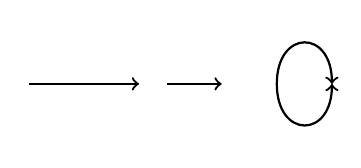
\begin{tikzpicture}[baseline=(current bounding box.center), scale=0.7]
        % Arrows
        \draw[myarrow] (-1,0) -- (1,0);
        \draw[myarrow] (1.5,0) -- (2.5,0);
        % Crossing
        \draw[myarrow] (3.5,0) .. controls (3.5,1) and (4.5,1) .. (4.5,0);
        \draw[myarrow] (3.5,0) .. controls (3.5,-1) and (4.5,-1) .. (4.5,0);
        \node[crossing] at (4,0) {};
    \end{tikzpicture}
};
\node at (even4) {
    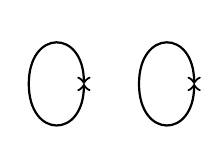
\begin{tikzpicture}[baseline=(current bounding box.center), scale=0.7]
        % Left curved arrow
        \draw[myarrow] (0,0) .. controls (0,1) and (1,1) .. (1,0);
        \draw[myarrow] (0,0) .. controls (0,-1) and (1,-1) .. (1,0);
        % Right curved arrow
        \draw[myarrow] (2,0) .. controls (2,1) and (3,1) .. (3,0);
        \draw[myarrow] (2,0) .. controls (2,-1) and (3,-1) .. (3,0);
    \end{tikzpicture}
};

% Odd row
\node at (odd1) {Odd};
\node at (odd2) {
    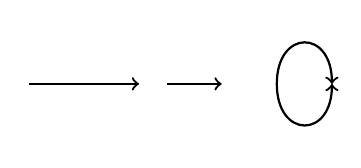
\begin{tikzpicture}[baseline=(current bounding box.center), scale=0.7]
        % Arrows
        \draw[myarrow] (-1,0) -- (1,0);
        \draw[myarrow] (1.5,0) -- (2.5,0);
        % Crossing
        \draw[myarrow] (3.5,0) .. controls (3.5,1) and (4.5,1) .. (4.5,0);
        \draw[myarrow] (3.5,0) .. controls (3.5,-1) and (4.5,-1) .. (4.5,0);
        \node[crossing] at (4,0) {};
    \end{tikzpicture}
};
\node at (odd3) {
    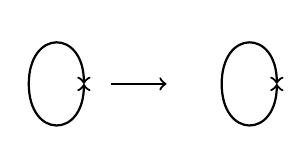
\begin{tikzpicture}[baseline=(current bounding box.center), scale=0.7]
        % Left curved arrow
        \draw[myarrow] (0,0) .. controls (0,1) and (1,1) .. (1,0);
        \draw[myarrow] (0,0) .. controls (0,-1) and (1,-1) .. (1,0);
        % Right arrow
        \draw[myarrow] (1.5,0) -- (2.5,0);
        % Right curved arrow
        \draw[myarrow] (3.5,0) .. controls (3.5,1) and (4.5,1) .. (4.5,0);
        \draw[myarrow] (3.5,0) .. controls (3.5,-1) and (4.5,-1) .. (4.5,0);
    \end{tikzpicture}
};
\node at (odd4) {
    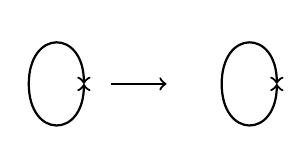
\begin{tikzpicture}[baseline=(current bounding box.center), scale=0.7]
        % Left curved arrow
        \draw[myarrow] (0,0) .. controls (0,1) and (1,1) .. (1,0);
        \draw[myarrow] (0,0) .. controls (0,-1) and (1,-1) .. (1,0);
        % Right arrow
        \draw[myarrow] (1.5,0) -- (2.5,0);
        % Right crossing
        \draw[myarrow] (3.5,0) .. controls (3.5,1) and (4.5,1) .. (4.5,0);
        \draw[myarrow] (3.5,0) .. controls (3.5,-1) and (4.5,-1) .. (4.5,0);
        \node[crossing] at (4,0) {};
    \end{tikzpicture}
};

% Add annotations
\node at ([xshift=-1cm]even2.east |- even2.south) {\textcolor{red}{R.H.}};

\end{tikzpicture}

\end{document}